\pagebreak
\section{Methods}
\label{ch:Methods}

\subsection{Method of approach}
The numerical modeling code, SNAC (\textbf{S}tGermai\textbf{N} \textbf{A}nalysis of \textbf{C}ontinua), is an explicit Lagrangian finite element code that solves the force and energy \add[XT]{find out which one is energy balance equation} balance equations for elasto-visco-plastic materials. Figure~\ref{fig_Methods7_3} shows major components of SNAC.

For each time step, strain and strain rates are updated based on the initial or previous velocity fields under the constraints from boundary conditions. A constitutive model returns updated stresses corresponding to these deformation measures. Internal forces are then calculated from the updated stresses, which is plugged into the momentum balance equation together with the body force term. Then, the damped \add[XT]{better understand the damped force} net force divided by inertial mass yields acceleration at a node point, which is time-integrated to velocity and displacement.

A 3D domain is discretized into hexahedral elements, each of which is in turn divided into two sets of tetrahedra. This symmetric discretization prevents faulting from favoring a specific direction or ``mesh grains''. 

Rheology for the oceanic lithosphere is assumed to be elasto-visco-plastic (EVP). When viscosity is high at low temperature, the EVP rheology implemented in SNAC essentially becomes the Mohr-Coulomb plasticity with strain softening that can create shear bands that behave like faults. Strain softening is realized by cohesion decreasing with increasing amount of permanent (i.e., plastic) strain. I assume this relationship is linear for simplicity. It is sufficient for a full description of such a linear strain weakening to define initial and final values of cohesion and a critical plastic strain at which cohesion becomes the final value. I define the rate of strain weakening as the cohesion difference divided by the critical plastic strain and use it as one of the model parameters. When temperature is high and viscosity is low, the rheology becomes the Maxwell viscoelasticity and can model creeping flow. This property of the EVP model makes it possible to set up a structure with a brittle lithosphere and a ductile asthenosphere through a proper temperature distribution. Rheological parameters are taken from previous studies that use a similar rheology [e.g., \citealp{Buck2005}; \citealp{Tucholke2008}] or from lab experiments \citep[e.g.,][]{Kirby1987}. 

For 3D diking processs, the strain $\Delta\varepsilon_{xx}$ associated with diking leads to stresses changes, $\Delta\sigma_{xx}$, $\Delta\sigma_{yy}$ and $\Delta\sigma_{zz}$. These stress changes due to diking are computed according to the linear elastic constitutive equations $\sigma_{ij}=\lambda\varepsilon_{kk}\delta_{ij}+2\mu\varepsilon_{ij}$.

\begin{figure}[H]
 \centering
%  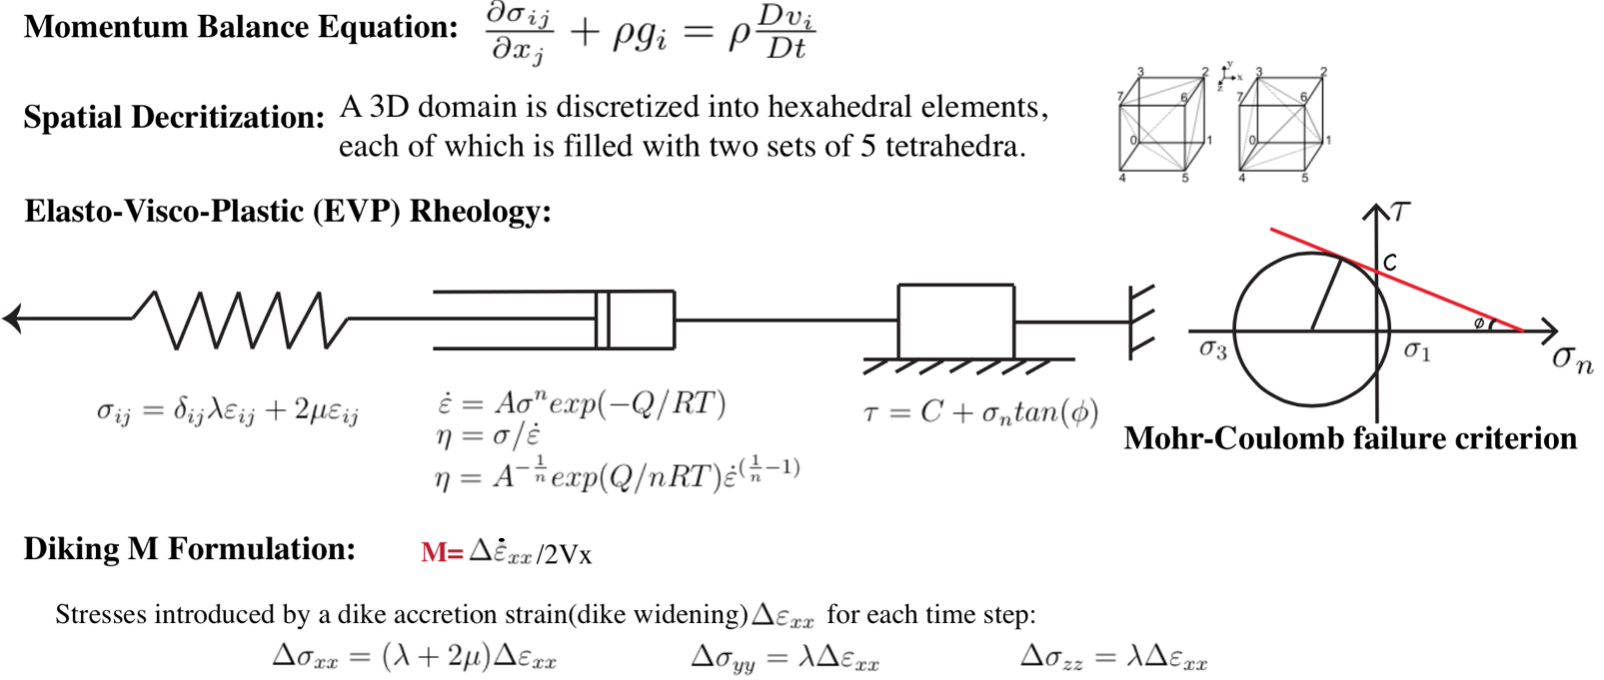
\includegraphics[scale=0.65]{fig_Methods7_2.png}
  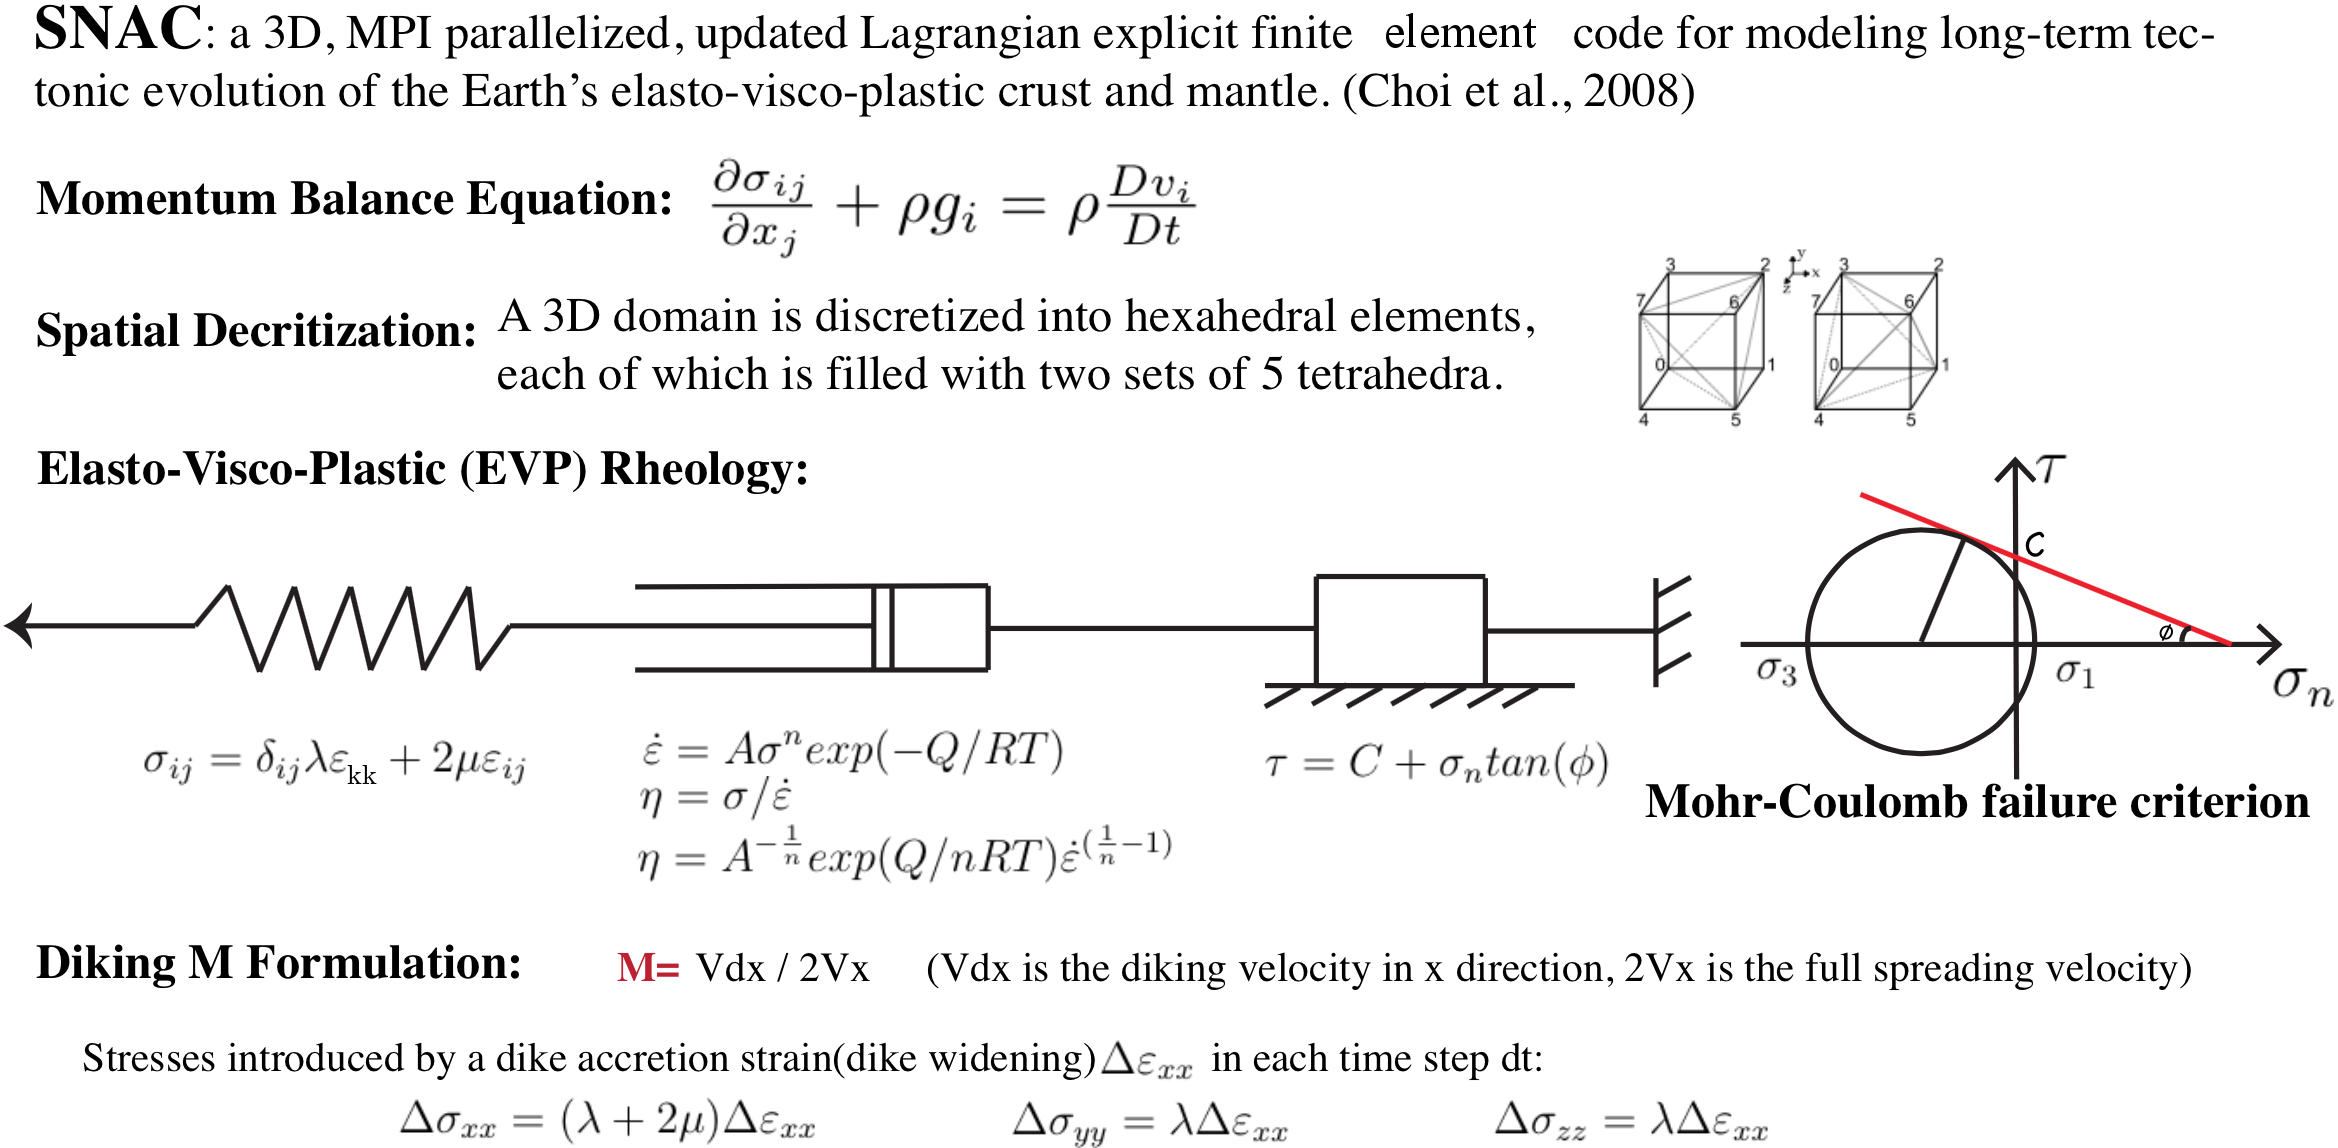
\includegraphics[width=1.0\textwidth]{./Figures/fig_Methods7_3.png}
 \caption{\small{Essential components of the numerical method.}}
 \label{fig_Methods7_3}
\end{figure}

\subsection{Model Setup}
The 3D models have a common geometry of 60 km $\times$ 20 km $\times$ 20 km in $x$, $y$ and $z$ axes \note[EC]{Correct the orientation of the coordinate axes. Y is vertically upward} respectively with a resolution ($\Delta x$) of 1 km (i.e., $\Delta x$ is the size of each hexahedron element). %For comparison with the previous 2D models \citep[e.g.][]{Buck2005, Tucholke2008}, I \note[EC]{also run pseudo-2D models}{Are you still going to include pseudo-2D models?} and they have a geometry of (60 km $\times$ 20 km $\times$ 1 km) in $x$, $y$ and $z$ axes respectively with a resolution of $\Delta x$ = 0.5 km.
The initial temperature field linearly increases from 0 \degree C at the top surface to 240 \degree C at the depth of 6 km, reflecting enhanced cooling due to hydrothermal circulation (Fig.~\ref{fig_Methods8_1}). Below 6 km, the temperature profile follows the semi-infinite half-space cooling model of moving plates \citep[e.g.,][]{Turcotte2002}. Two sides perpendicular to the $z$ coordinate axis are free-slip. The top surface has vertical tractions from water columns, of which heights are locally determined as (4000 - $h(x,z)$) m, where $h(x,z)$ is the topography at a location, $(x,z)$. The bottom surface is supported by the Winkler foundation. Temperature is fixed at 0 \degree C on the top surface and at 1300 \degree C on the bottom surface. 

Diking, represented by the factor M as described above, is assumed to occur in the middle of the doamin (Fig.~\ref{fig_Methods8_1}), where lithosphere is thinnest.

We adopt the linear isotropic elasticity, power-law viscosity of dry diabase \citep[e.g.,][]{Kirby1987, Buck2005} and the Mohr-Coulomb plastic model. The complete list of model parameters are given in Table~\hyperref[Tab_ModelParameters]{\ref{Tab_ModelParameters}}.

\begin{figure}[H]
 \centering
%  \includegraphics[scale=0.55]{fig_Methods8_1.png}
  \includegraphics[width=1.0\textwidth] {./Figures/fig_Methods8_1.png}
 \caption{\small Model setup}
 \label{fig_Methods8_1}
\end{figure}


\begin{table}[h]
\caption{Summary of 3D Model Parameters}
\centering
 \small
  \begin{tabular}[h]{l l p{6.8cm} l l}
\hline
\hline
Number & Variable & Description & Value & Units \\ 
\hline
1    &  $W_{dike}$    &   Dike width        & 2   &  $km$\\
\hline
2    &  $D_{dike}$    &   Dike depth        & 8   &  $km$\\
\hline
3    &  $H$    &   Crustal thickness at dike   & 6   &  $km$ \\
\hline
4    &  $dT/dy$    &   Crustal thermal gradient        & 40   &  $K/km$ \\
\hline
5    &  $T_{1}$    &   Temperature at lower boundary of crust    & 240   &  $\degree C$ \\
\hline
6    &  $g$    &   Gravity acceleration    & 10   &  $m/s^{2}$ \\
\hline
7    &  $demf$    &   Dimensionless force damping factor   & 0.8   &  N/A  \\
\hline
8    &  $dt$    &   Time step    & 1.5768e+07   &  $second$  \\
\hline
9    &  $topo_kappa$    &   Parameter for topography smoothing    & 0   &  N/A   \\
\hline
10   &  $shadowDepth$    &   Ghost elements for parallel computing   & 2   &  N/A   \\
\hline
11   &  $meshI$    &   Mesh number in X direction   & 60   &  N/A   \\
\hline
12   &  $meshJ$    &   Mesh number in Y direction      & 20   & N/A  \\
\hline
13   &  $meshK$    &   Mesh number in Z direction      & 20   & N/A  \\
\hline
14   &  $L_{I}$    &   Length in X direction      & 20   & $km$  \\
\hline
15   &  $L_{J}$    &   Length in Y direction      & 20   & $km$  \\
\hline
16   &  $L_{K}$    &   Length in Z direction      & 20   & $km$  \\
\hline
17   &  $\rho$    &    Density      & 3000   & $kg/m^{3}$  \\
\hline
18   &  $\lambda$    &    Lam$\acute{e}$'s constant      & 30   & $Gpa$  \\
\hline
19   &  $\mu$    &    Shear modulus      & 30   & $Gpa$  \\
\hline
20   &  $refvisc$    &    Reference viscosity      & 0.125e-17   & $Pa^{-n}/s$  \\
\hline
21   &  $activationE$    &    Activation Energy      & 276.0e+3   & $kJ/mol$  \\
\hline
22   &  $vis_{min}$    &    viscosity minimum cutoff      & 1.0e+18   & $Pa*s$  \\
\hline
23   &  $vis_{max}$    &    viscosity maximum cutoff      & 1.0e+27   & $Pa*s$  \\
\hline
24   &  $srexponent$    &    Power of power law in viscosity       & 3.05   & N/A  \\
\hline
25   &  $\varepsilon_{p_{i}}^{1}$    &    initial plastic strain for piecewise Type 1 weakening       & $0$   & N/A  \\
\hline
26   &  $\varepsilon_{p_{i}}^{2}$    &    initial plastic strain for piecewise Type 2 weakening       & $0$   & N/A  \\
\hline
27   &  $\varepsilon_{p_{e}}^{1}$    &    end plastic strain for piecewise Type 1 weakening       & $0.1$   & N/A  \\
\hline
28   &  $\varepsilon_{p_{e}}^{2}$    &    end plastic strain for piecewise Type 2 weakening       & $0.33$   & N/A  \\
\hline
29   &  $C_{i}$    &    initial Cohesion for piecewise weakening       & 44   & $Mpa$  \\
\hline
30   &  $C_{e}$    &    end Cohesion for piecewise weakening       & 4   & $Mpa$  \\
\hline
31   &  $\phi$    &    Friction angle      & 30   & $\degree$  \\
\hline
32   &  $remesh_{timestep}$    &    Remesh when timestep reach its value      & 400000   & N/A  \\
\hline
33   &  $remesh_{length}$    &    Remesh when the global minimum of the ratio of the volume of a tetrahedron to one of its surface area      & 0.6   & N/A  \\
\hline
34   &  $top_{Temp}$    &    Surface temperature      & 0   & $\degree C$  \\
\hline
35   &  $bottom_{Temp}$    &    Bottom temperature      & 1300   & $\degree C$  \\
\hline
36   &  $V_{x}$    &    Half spreading rate      & 7.9e-10   & $m/s$  \\

\hline
\hline
\end{tabular}

\label{Tab_ModelParameters}
\end{table}

\subsection{Parameters to control}
Before running 3D models, I have run hundreds of psedudo-2D models for initial setup and benchmarking with previous studies \citep[e.g.,][]{Buck2005, Tucholke2008}. Preliminary pseudo-2D results show that the model behavior in faulting pattern is sensitive to the rate of strain weakening. Two cases of strain weakening are tested in the 3D models. In one case (denoted as Type 1 weakening), cohesion linearly decreases from 44 MPa (denoted as $C_{i}$) to 4 MPa ($C_{e}$) for plastic strain accumulating from 0 ($\varepsilon_{p_{i}}^{1}$) to 0.1 ($\varepsilon_{p_{e}}^{1}$). It has a characteristic fault slip of 150 m for pseudo-2D models and 300 m for 3D models. The other case (Type 2 weakening) assumes cohesion linearly decreasing from 44 MPa ($C_{i}$) to 4 MPa ($C_{e}$) for plastic strain accumulating from 0 ($\varepsilon_{p_{i}}^{2}$) to 0.33 ($\varepsilon_{p_{e}}^{2}$). In this case, the characteristic fault slip for pseudo-2D models is 500 m and for 3D models is 1 km. The characteristic fault slip is defined as $\Delta X_{c}$=3$\Delta x \varepsilon_{p_{e}}$ where 3 $\Delta x$ represents the thickness of the shear bands which is usually 2 to 4 times $\Delta x$ (size of a hexahedron element) \citep{Lavier2000}. When $\Delta X_{c}$ amount of slip takes place at the fault interface, the cohesion of the material at the faulting interface decreases to $C_{e}$. In this way, under the same amount of $\Delta X_{c}$, models with different resolution should produce the same faulting patterns. 

Meanwhile, although how to estimate the M values from observations is a subject of on-going research, we do have constraints from a large dataset of bathymetry, gravity and seismic surveys as well as geological drilling. Generally, at slow spreading ridges, magma supplies mostly at the center of the ridge segment and decreases towards the tip of the segment \citep{Tolstoy1993,Chen1999,Carbotte2015}. There is also evidence for shorter wavelength of 10 to 20 km discrete focus of magma accretion along the ridge axis \citep{Lin1990}. Based on these constraints, I start considering a few scenarios of variations in M along the ridge axis. They are three M ranges (i.e. 0.2$\sim$0.8 (M28), 0.5$\sim$0.7 (M57) and 0.5$\sim$0.8 (M58)) with three simple functional forms of M variations (i.e. linear, sinusoidal and square root).

The numerical cost of a 3D model is non-trivial. For 2 Myr of model time, each model usually runs on 192 cores for about 48 hours (i.e., around 10$^{4}$ core-hours). %\add[XT]{use 96 cores can improve the efficiency a little bit (Longer time but smaller amount of SUs needed).})
Under this constraint of computational cost, I control only the following three parameters while fixing all the others: 1) there types of functionalforms (i.e. linear, sinusoidal and square root); 2) three ranges of M variation along the ridge axis (0.5$\sim$0.7 (M57); 0.5$\sim$0.8 (M58); 0.2$\sim$0.8 (M28)) and 3) two types of weakening rate (Type 1 and Type 2).

Till now, 11 $+$ 1 3D models are run (11 models with M varying along the ridge-axis and 1 model with constant M = 0.8. The complete list of 3D models is given in Table~\hyperref[Tab1_1]{\ref{Tab1_1}}. 

\begin{table}[h]
\centering
\begin{tabular}{l l l l l}
\hline
\hline
Model& M range & Functional Form & Type of weakening & For short \\ 
\hline
1    &  M28    &   Linear        & Type 1   &  M28LinT1\\
\hline
2    &  M28    &   Sinusoidal    & Type 1   &  M28SinT1\\
\hline
3    &  M28    &   Square Root   & Type 1   &  M28SqrtT1 \\
\hline
4    &  M57    &   Linear        & Type 1   &  M57LinT1 \\
\hline
5    &  M57    &   Sinusoidal    & Type 1   &  M57SinT1 \\
\hline
6    &  M57    &   Sinusoidal    & Type 2   &  M57SinT2 \\
\hline
7    &  M57    &   Square Root   & Type 2   &  M57SqrtT2  \\
\hline
8    &  M58    &   Sinusoidal    & Type 1   &  M58SinT1  \\
\hline
9    &  M58    &   Sinusoidal    & Type 2   &  M58SinT2   \\
\hline
10   &  M58    &   Square Root   & Type 1   &  M58SqrtT1   \\
\hline
11   &  M58    &   Square Root   & Type 2   &  M58SqrtT2   \\
\hline
12   &  M88    &   Constant      & Type 2   &  M88ConT2 \\
\hline
\hline
\end{tabular}
\caption{List of 3D numerical experiments.}
\label{Tab1_1}
\end{table}




